\card{Softwarearchitektur und Patterns}{
	Die Architektur eines Softwaresystems definiert dieses System in Bezug auf rechnerische Komponenten und Interaktionen zwischen diesen Komponenten. Es involviert eine Beschreibung von Elementen aus denen das System gebaut wird, Interaktionen zwischen ihren Elementen, Patterns, die ihre Zusammensetzung führen und Einschränkungen dieser Patterns.
}

\card{Softwarearchitektur und Patterns (architektonische Stile)}{
	\begin{compactenum}
		\item pipe and filter
		\item call and return (empfohlen: high fan-in, low fan-out)
		\item Layers in hierarchischer Architektur (Layer: Gruppe von eng verwandten und sehr verbundenen Funktionalitäten)
		\item blickdichtes Layering: vm kann nur vom unterliegenden Layer aufgerufen werden (Aufteilung von Bedenken, Wartbarkeit, Flexibilität)
		\item transparentes Layering: vm kann von jedem anderen Layer aufgerufen werden (Laufzeiteffizienz (keine Parameter/Weitergabe von Nachrichten, Datenkonversation, Formatänderungen))
		\item Client/Server (Kommunikation von Empfängern) - Client: Prozess, der auf Daten zugreifen/Ressourcen benutzen/Operationen ausführen möchte, Server: Prozess, der Daten und gemeinsam genutzte Ressourcen managed
	\end{compactenum}
}

\card{Softwarearchitektur und Patterns (architektonische Stile: pipe and filter)}{
	\scalebox{0.85}{\input{pictures/pipeandfilter.pgf}}
}
\card{Softwarearchitektur und Patterns (architektonische Stile: call and return)}{
	\scalebox{1}{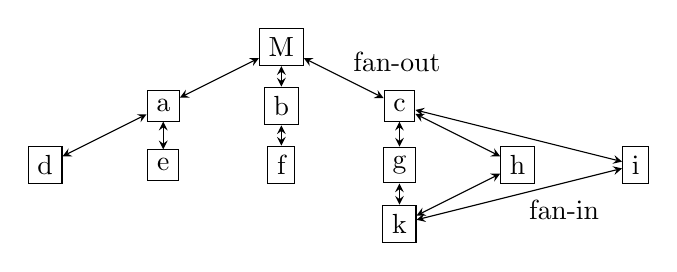
\begin{tikzpicture}[
>=stealth,
every path/.style={draw,<->},
node distance=1.5cm
]

%\node (text) at (-2.2,0) {call and return:};
\node[draw] (root) at (0,0) {M};
	\node[draw] (b) [below of = root,yshift=0.75cm] {b};
		\node[draw] (f) [below of = b,yshift=0.75cm] {f};
	\node[draw] (a) [left of = b] {a};
		\node[draw] (e) [below of = a,yshift=0.75cm] {e};
		\node[draw] (d) [left of = e] {d};
	\node[draw] (c) [right of = b] {c};
		\node[draw] (g) [below of = c,yshift=0.75cm] {g};
			 \node[draw] (k) [below of = g,yshift=0.75cm] {k};
		\node[draw] (h) [right of = g] {h};
		\node[draw] (i) [right of = h] {i};

\path (root) -- (a);
	\path (a) -- (d);
	\path (a) -- (e);
\path (root) -- (b);
	\path (b) -- (f);
\path (root) to node [right,yshift=0.2cm]  {fan-out} (c);
	\path (c) -- (g);
	\path (c) -- (h);
	\path (c) -- (i);
		\path (g) -- (k);
		\path (h) -- (k);
		\path (i) to node [right,yshift=-0.2cm]  {fan-in} (k);

\end{tikzpicture}}
}

\card{Softwarearchitektur und Patterns (architektonische Stile: Layers in hierarchischer Architektur)}{
	\scalebox{0.8}{\input{pictures/vertpart.pgf}}\\\ \\
	\scalebox{0.8}{\input{pictures/horpart.pgf}}
}